\subsection{Framework vs Bibliothek}
\begin{flushleft}
  In dieser Arbeit stehen ein Framework und eine Bibliothek zur Auswahl.
  \\
  Beide Technologien, sowohl React als auch Angular, wurden für die Entwiklung von SPAs\footnote{Single-page application {\cite{MO1}}} konzipiert.

  Eine Bibliothek wie React bietet mehr Kontroll darauf, wie der Code entwickelt werden kann und erlaubt Applikationen mit anderer Bibliotheken zu erweitern. Für das State-Management wird zum Beispiel häufig Redux{\cite{RE1}} verwendet.

  Andererseits das Framework von Angular gibt genauer vor, wie der Code entwickelt werden muss\footnote{{\cite{AN1}}, Seite 27}.
  \\
  In dieser Arbeit wird nicht näher auf den Unterschied zwischen einer Bibliothek und einem Framework eingegangen, da beide die Anforderungen des Projekts abdecken.
\end{flushleft}

\subsubsection{GraphQL Playground}
Mit GraphQL Playground haben wir die Möglichkeit, alle Abfragen und Mutationen zu testen. Wir erhalten Zugriff auf relevante Informationen wie verfügbare Felder und deren Datentyp. Diese Informationen werden aktualisiert, wenn der Servercode geändert wurde. Dadurch wurde eine aktuelle API-Dokumentation gewährleistet. Für unser Projekt war es sehr praktisch und hat die Kommunikation als Entwickler effizienter gemacht.
\\
\begin{center}
%  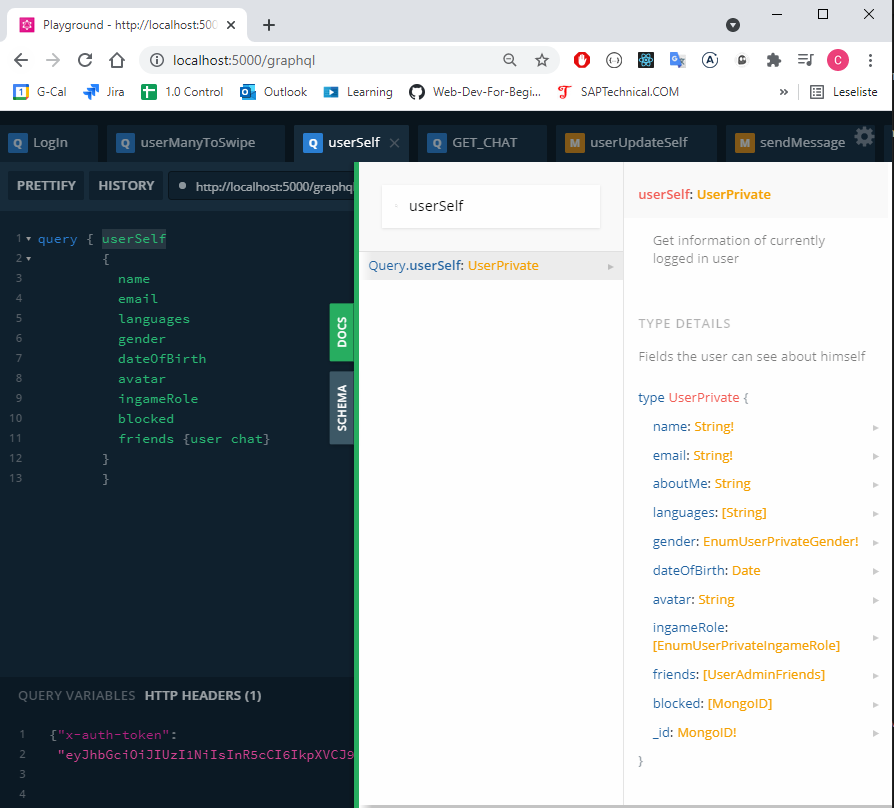
\includegraphics[scale=0.60]{GraphQL_Playground}\label{fig:GraphQL_Playground}
\end{center}
\textbf{Abbildung \autoref{fig:GraphQL_Playground}:}
%Genau derselbe Code wird für die Abfrage von Benutzerinformationen später verwendet.
\newpage

\subsection{Implementierung der Serverabfragen mit GraphQL}
Alle Abfragen und Mutationen wurden in einem separaten Ordner gesammelt.
Damit soll eine saubere Struktur des Codes gewährleistet werden.
Diese wurden für die spätere Verwendung in den React-Komponenten exportiert.

Mithilfe der Hooks useQuery bzw. useMutation von Apollo Client wurden die Lese- und Schreibabfragen durchgeführt.
\\\\
\textbf{Apollo Client}\\
Warum haben wir uns für Apollo entschieden? Was ist ApolloClient?
TODO
%Coming...
\newpage

\subsubsection{Leseabfrage}
Nachdem eine Abfrage exportiert wurde, ist sie bereit, in einer React-Komponente \\
importiert und angewendet zu werden.

\begin{lstlisting}
import { GET_MY_INFO } from "./GraphQL/Queries"
import { useQuery } from "@apollo/client"

const { loading, error, data } = useQuery(
GET_MY_INFO,
ContextHeader(token),
)
//Code-Auszug in frontend/src/App.js

\end{lstlisting}
Die Konstante ContextHeader enthält das Token in der Struktur, die erforderlich ist, um die Abfrage nur dann stellen zu können, wenn der Benutzer dazu berechtigt ist.
\\
Sollte das Token einen undefinierten Wert, null oder ungültig enthalten, wird der Server ein Fehler zurückgegeben.
\\
Der useQuery Hook liefert ein Ergebnisobjekt, welches eine der folgenden Optionen zurückgibt.
\\\\
\textbf{loading:}\\
Ein boolescher Wert, der angibt, ob die Abfrage in Bearbeitung ist.
Wenn loading wahr ist, ist die Anfrage noch nicht abgeschlossen. Typischerweise kann diese Information verwendet werden, um einen Lade-Spinner anzuzeigen.
\\\\
\textbf{error:}\\
Ein Laufzeitfehler mit den Eigenschaften von GraphQL Errors und network Error.
Dieses enthält Informationen darüber, was bei der Abfrage fehlgeschlagen  ist.
\\\\
\textbf{date:}\\
Ein Objekt, das das Ergebnis der GraphQL-Abfrage enthält.
\\Es enthält die tatsächlichen Daten vom Server.
\newpage
\subsection{Axios}
\begin{comment}
\begin{quote}
  Axios ist ein Promise-basierter HTTP-Client für node.js und den browser. Auf der Server-Seite wir das modul HTTP verwendet, während im Browser XMLHttpRequests (ajax) ausgeführt werden.
\end{quote}\footnote{Vgl. u.a. \cite{AX1}}
\end{comment}

Zusätzlich zu den GraphQL-Abfragen wurde eine Post-Anfrage mit Axios bereitgestellt.
Mit dieser war es möglich, Bilder auf eine S3 Speichereinheit von Amazon Web Services hochzuladen.
\\
Ein Auszug aus dem zu diesem Zweck verwendeten Code findet sich in Anhang 4.

%Das HTML-Eingabefeld „input“ wurde folgendermaßen definiert.
%\begin{lstlisting}
%   <input type="file" onChange={fileSelectedHandler} />
%\end{lstlisting}

\begin{flushleft}
Das Format der hochzuladenden Dateien wurde auf .png, .jpg und .jpeg beschränkt, damit nur zulässige Dateien an den Server gesendet werden.
\\
Die Größe der hochzuladenden Datei wurde um 1 MB abgegrenzt.
\end{flushleft}
